\section{Theory} \label{sec:theory}
Regression analysis are widely used in different fields of natural sciences, data science and economics to mention some. The simplest form is the linear regression, which is intuitive and easy to work with. 
 
\subsection{Linear regression} \label{sec:regression}
In linear regression, the dependent variable $y_i$ is a linear combination of the parameters. \cite{hastie01statisticallearning}

\subsubsection{Ordinary Least Square (OLS)} \label{sec:OLS}
Suppose we have a set of points $\{(x_1, y_1), (x_2, y_2),\hdots, (x_n, y_n)\}$, and we want to fit a p'th order polynomial to them. The most intuitive way would be to find coefficients $\vec{\beta}$ which minimize the error in
\begin{align*}
y_1&=\beta_0x_1^0+\beta_1x_1^1+\hdots+\beta_px_1^p+\varepsilon_1\\
y_2&=\beta_0x_2^0+\beta_1x_2^1+\hdots+\beta_px_2^p+\varepsilon_2\\
\vdots\\
y_n&=\beta_0x_n^0+\beta_1x_n^1+\hdots+\beta_px_n^p+\varepsilon_n,
\end{align*}

Instead of dealing with a set of equations, we can apply linear algebra. One can easily see that the equations above correspond to
\begin{equation}
\vec{y}=\hat{X}^T\vec{\beta}+\vec{\varepsilon},
\label{eq:y_xb}
\end{equation}
with
\begin{equation}
\hat{X}=\begin{pmatrix}
x_1^0&x_1^1&x_1^2&\hdots&x_1^p\\
x_2^0&x_2^1&x_2^2&\hdots&x_2^p\\
\vdots&\vdots&\vdots&\ddots&\vdots\\
x_n^0&x_n^1&x_n^2&\hdots&x_n^p
\end{pmatrix}
\end{equation}
as the \textit{design} matrix and
\begin{equation}
\vec{\beta}=(\beta_0, \beta_1, \hdots, \beta_p)
\end{equation}
as the coefficients. 

For a nonsingular matrix $\hat{X}$ (but not necessary symmetric) we can find the optimal $\vec{\beta}$ by solving
\begin{equation}
\vec{\beta}=(\hat{X}^T\hat{X})^{-1}\hat{X}^T\vec{y},
\end{equation}
which again corresponds to minimizing the cost function,
\begin{equation}
\vec{\beta}=\text{argmin},\vec{\beta}\bigg\{\sum_{i=1}^{n}\Big(y_i-\beta_0-\sum_{j=1}^px_{ij}\beta_j\Big)^2\bigg\}.
\end{equation}
where we here have used the standard cost function, given by least squares,

\begin{equation}
Q(\vec{\beta})=\sum_{i=1}^{n}(y_i-\tilde{y}_i)^2=(\vec{y}-\hat{X}\vec{\beta})^T(\vec{y}-\hat{X}\vec{\beta}).
\end{equation}

This works perfectly when all rows in $\hat{X}$ are linearly independent, but this will generally not be the case for large data sets. If we are not able to diagonalize the matrix, we will not be able to calculate $(\hat{X}^T\hat{X})^{-1}$, so we need to do something smart. 

Fortunately there is a simple trick we can do to make all matrices diagonalizable; we can add a diagonal matrix to the initial matrix. 


\subsubsection{Ridge regression} \label{sec:ridge}
Ridge regression is a widely used method that can handle singularities in matrices. The idea is to modify the standard cost function by adding a small term,
\begin{equation}
Q^{\text{ridge}}(\vec{\beta})=\sum_{i=1}^N(y_i-\tilde{y_i})^2+\lambda||\vec{\beta}||_2^2,
\end{equation}
where $\lambda$ is the so-called \textit{penalty} and $||\vec{v}||_2$ is defined as
\begin{equation}
||\vec{v}||_2=\sqrt{\vec{v}^T\vec{v}}=\Big(\sum_{i=1}^Nv_i^2\Big)^{1/2}.
\end{equation}
This will eliminate the singularity problem.

Further we find the optimal $\vec{\beta}$ values by minimizing the function 
\begin{equation}
\vec{\beta}^{\text{ridge}}=\text{argmin},\vec{\beta}\bigg\{\sum_{i=1}^{n}\Big(y_i-\beta_0-\sum_{j=1}^px_{ij}\beta_j\Big)^2+\lambda\sum_{j=1}^p\beta_j^2\bigg\}, 
\end{equation}
or we could simply solve the equation
\begin{equation}
\vec{\beta}^{\text{ridge}}=(\hat{X}^T\hat{X}+\lambda I)^{-1}\hat{X}^T\vec{\beta}.
\end{equation}
In the latter equation we can easily see why this solves our problem.

\subsubsection{Lasso regression} \label{sec:lasso}
The idea behind Lasso regression is similar to the idea behind Ridge regression, and they differ only by the exponent factor in the last term. The modified cost function now writes
\begin{equation}
Q^{\text{lasso}}(\vec{\beta})=\sum_{i=1}^N(y_i-\tilde{y_i})^2+\lambda||\vec{\beta}||_2,
\end{equation}
and to find the optimal coefficients $\vec{\beta}$, we need to minimize
\begin{equation}
\vec{\beta}^{\text{lasso}}=\text{argmin},\vec{\beta}\bigg\{\sum_{i=1}^{n}\Big(y_i-\beta_0-\sum_{j=1}^px_{ij}\beta_j\Big)^2+\lambda\sum_{j=1}^p|\beta_j|\bigg\}.
\end{equation}

\subsubsection{General form} \label{sec:general}
We can generalize the models above to a minimization problem where we have a $q$ in the last exponent, 
\begin{equation}
\vec{\beta}^q=\text{argmin},\vec{\beta}\bigg\{\sum_{i=1}^{n}\Big(y_i-\beta_0-\sum_{j=1}^px_{ij}\beta_j\Big)^2+\lambda\sum_{j=1}^p|\beta_j|^q\bigg\},
\end{equation}
such that $q=2$ corresponds to the Ridge method and $q=1$ is associated with Lasso regression. It can also be interesting to try other $q$-values.

\subsection{Multivariate linear regression} \label{sec:higher_reg}
We can use the same approach as above when dealing with regression of higher order, since the problem is to fit a function to points, no matter how many components they have. We will first take a look at how we can fit a 2D polynomial to some terrain data, before we briefly describe how to fit a function of arbitrary order to points.

\subsubsection{Terrain} \label{sec:terrain}
A set of data points $\{(x_1, y_1, z_1), (x_2, y_2, z_2),\hdots, (x_n, y_n,z_n)\}$ gives some coordinates in space, which for instance can describe the terrain. The system of linear equations to solve can then be lined up as 
\begin{align*}
z_1&=\beta_0x_1^0y_1^0+\beta_1x_1^1y_1^0+\beta_2x_1^0y_1^1+\hdots+\beta_{p^2}x_1^py_1^p+\varepsilon_1\\
z_2&=\beta_0x_2^0y_2^0+\beta_1x_2^1y_2^0+\beta_2x_2^0y_2^1+\hdots+\beta_{p^2}x_2^py_2^p+\varepsilon_2\\
\vdots\\
z_n&=\beta_0x_n^0y_n^0+\beta_1x_n^1y_n^0+\beta_2x_n^0y_n^1+\hdots+\beta_{p^2}x_n^py_n^p+\varepsilon_n,
\end{align*}
when fitting a polynomial of p'th order. In general the order associated with x-direction do not need to be the same as the order associated with y-direction. 

We can set up a similar equation as for the first order case, presented in equation \eqref{eq:y_xb}, but we will now (typically) have $\vec{z}$ on the left hand side and $\hat{X}$ will contain both x- and y-coordinates:
\begin{equation}
\vec{z}=\hat{X}^T\vec{\beta}.
\end{equation}
The design matrix $\hat{X}$ will now look like
\begin{equation}
\hat{X}=
\begin{pmatrix}
x_1^0y_1^0&x_1^1y_1^0&x_1^0y_1^1&x_1^1y_1^1&\hdots&x_1^py_1^p\\
x_2^0y_2^0&x_2^1y_2^0&x_2^0y_2^1&x_2^1y_2^1&\hdots&x_2^py_2^p\\
\vdots&\vdots&\vdots&\vdots&\ddots&\vdots\\
x_n^0y_n^0&x_n^1y_n^0&x_n^0y_n^1&x_n^1y_n^1&\hdots&x_n^py_n^p
\end{pmatrix}
\end{equation}
and we can again use the OLS method to find $\vec{\beta}$, i.e, calculating
\begin{equation}
\vec{\beta}=(\hat{X}^T\hat{X})^{-1}\hat{X}^T\vec{z}.
\end{equation}
Similarly, we can use Ridge and Lasso regression in the same way as when fitting 1D polynomials. 

In this project we will actually deal with terrain data. Firstly, we implement some regression tools which fit a 2D function to points in space. To verify the implementation, we pick points from a known function such that we know the result. The specific verification function used is the Franke Function, which looks like

\begin{align*}
f(x,y) &= \frac{3}{4}\exp{\left(-\frac{(9x-2)^2}{4} - \frac{(9y-2)^2}{4}\right)}+\frac{3}{4}\exp{\left(-\frac{(9x+1)^2}{49}- \frac{(9y+1)}{10}\right)} \\
&+\frac{1}{2}\exp{\left(-\frac{(9x-7)^2}{4} - \frac{(9y-3)^2}{4}\right)} -\frac{1}{5}\exp{\left(-(9x-4)^2 - (9y-7)^2\right) },
\end{align*}
and is a smooth 2D function as one can see in figure \eqref{fig:data}, part (a).

 \begin{figure} [H]%
    \centering
    \subfloat[Franke function]{{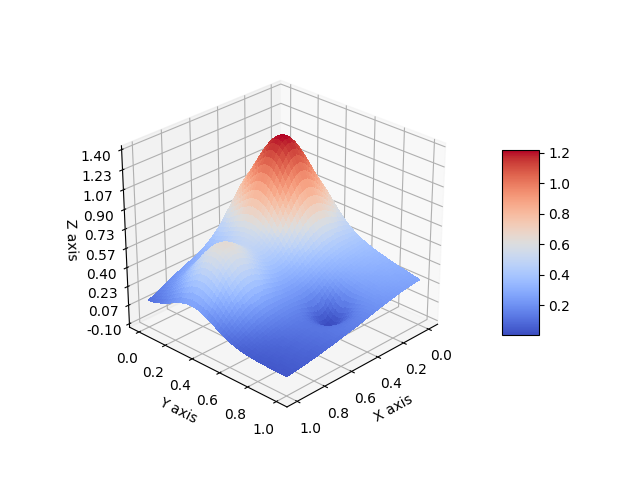
\includegraphics[width=8cm]{../plots/franke.png} }}%
    \subfloat[Lombok terrain]{{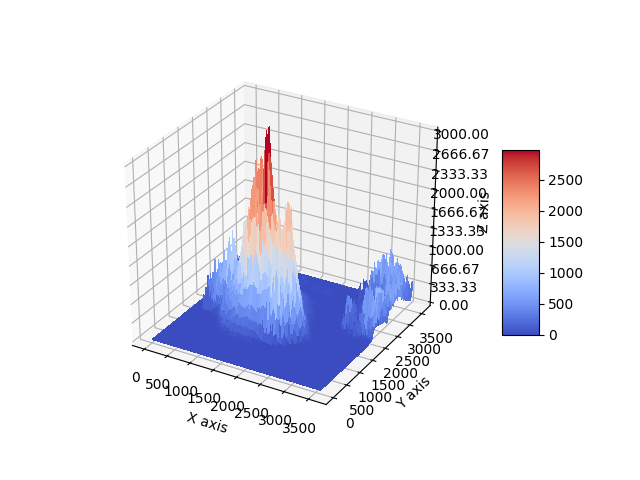
\includegraphics[width=8cm]{../plots/lombok.png} }}
    \caption{The two data sets we are going to fit polynomials to.}%
    \label{fig:data}%
 \end{figure}

Secondly, we use the verified regression tools to fit a polynomial to real terrain data. The data is taken from United States Geological Survey (USGS) \url{https://earthexplorer.usgs.gov/}, and for investigation we picked the volcanic island of Lombok. Despite the island's small extent, it houses the second highest volcano in Indonesia which makes the terrain data interesting. See part (b) of figure \eqref{fig:data} for terrain data.

\subsubsection{Higher order}
There should be no surprise that we can extend the theory above to even higher orders. 
Although we stick to 2D regression in this project, we add this section for completeness. 

Suppose now that we have a data set of $n$ points in $d$ dimensions, \\ $\{(x_1^1, x_1^2, \hdots, x_1^d), (x_2^1, x_2^2,\hdots, x_2^d),\hdots, (x_n^1, x_n^2,\hdots,x_n^d)\}$, where the superscript indicates in which dimension the coordinate is, and the subscript is the coordinate number. We want to fit the points with a polynomial of degree $p\in\mathbb{R}^d$, where we assume that the fitting polynomial has the same degree in all direction, which makes the notation neater, but is not essential. To be more specific, we want polynomial coefficients $\vec{\beta}=(\beta_0, \beta_1, \hdots, \beta_{p^d})$ that minimizes the error in 
\begin{align*}
x_1^d&=\beta_0(x_1^1)^0(x_1^2)^0\hdots(x_1^d)^0 +\beta_1(x_1^1)^1(x_1^2)^0\hdots(x_1^d)^0+\hdots+\beta_{p^d}(x_1^1)^p(x_1^2)^p\hdots(x_1^d)^p+\varepsilon_1\\
x_2^d&=\beta_0(x_2^1)^0(x_2^2)^0\hdots(x_2^d)^0 +\beta_1(x_2^1)^1(x_2^2)^0\hdots(x_2^d)^0+\hdots+\beta_{p^d}(x_2^1)^p(x_2^2)^p\hdots(x_2^d)^p+\varepsilon_2\\
\vdots\\
x_n^d&=\beta_0(x_n^1)^0(x_n^2)^0\hdots(x_n^d)^0 +\beta_1(x_n^1)^1(x_n^2)^0\hdots(x_n^d)^0+\hdots+\beta_{p^d}(x_n^1)^p(x_n^2)^p\hdots(x_n^d)^p+\varepsilon_n.
\end{align*}
This gives a design matrix

\begin{equation}
\hat{X}=
\begin{pmatrix}
(x_1^1)^0(x_1^2)^0\hdots(x_1^d)^0&\hdots& (x_1^1)^1(x_1^2)^0\hdots(x_1^d)^0&\hdots&(x_1^1)^p(x_1^2)^p\hdots(x_1^d)^p\\
(x_2^1)^0(x_2^2)^0\hdots(x_2^d)^0&\hdots& (x_2^1)^1(x_2^2)^0\hdots(x_2^d)^0&\hdots&(x_2^1)^p(x_2^2)^p\hdots(x_2^d)^p\\
\vdots&\vdots&\vdots&\ddots&\vdots\\
(x_n^1)^0(x_n^2)^0\hdots(x_n^d)^0&\hdots& (x_n^1)^1(x_n^2)^0\hdots(x_n^d)^0&\hdots&(x_n^1)^p(x_n^2)^p\hdots(x_n^d)^p,
\end{pmatrix}
\end{equation}
and we can find the optimal $\vec{\beta}$ in the same way as above. 

\subsection{Some statistics} \label{sec:statistics}
When dealing with data sets, we always want to know how much the data points vary from each other, in other words we want to calculate the variance of the data. The variance from one data set is given by 
\begin{equation}
\sigma_y^2=\frac{1}{N}\sum_{i=1}^N(y_i-\bar{y})^2
\end{equation}
where the sample mean is given by
\begin{equation}
\bar{y}=\sum_{i=1}^Ny_i.
\end{equation}
We will stress that sample mean is not necessarily the same as the distribution mean, but the sample mean will approximate the distribution mean for large data sets. 

Often we are studying multiple data sets at the same time, and want to estimate the total variance. The sample mean of one data set $\alpha$ is still given by
\begin{equation}
\bar{y}_{\alpha}=\frac{1}{N}\sum_{i=1}^Ny_{\alpha,i},
\end{equation}
which for $M$ data sets gives a total sample mean of
\begin{equation}
\bar{y}_M=\frac{1}{M}\sum_{\alpha=1}^M\bar{y}_{\alpha}=\frac{1}{MN}\sum_{\alpha=1}^M\sum_{i=1}^Ny_{\alpha,i}.
\end{equation}
The total variance will then be a sum over the single set variances plus the cross terms
\begin{equation}
\sigma_M^2=\frac{1}{M}\sum_{\alpha=1}^M\frac{\sigma_{\alpha}^2}{N}+\frac{2}{MN^2}\sum_{\alpha=1}^M\sum_{i<j}^N(y_{\alpha,i}-\bar{y}_M)(y_{\alpha,j}-\bar{y}_M).
\end{equation}
The last term is called the covariance, and is a measure of how much the data set are related. If they are totally independent, the covariance is zero. For large data sets this term is computational expensive to calculate, and we will rather use resampling techniques to estimate the variance. A few resampling techniques are presented in the Method section.

\subsection{Error analysis} \label{sec:error_analysis}
Different methods to estimate error:
\begin{itemize}
	\item{Absolute error}
	\item{Relative error}
	\item{Mean square error (MSE)}
	\item{R$^2$ score function}
\end{itemize}
In this report we will study only the MSE and R$^2$ score function.

\subsubsection{Mean Square Error (MSE)} \label{sec:MSE}
The most popular error estimation method is the mean square error, also called least squares. \cite{hastie01statisticallearning} We study the MSE in order to find out how the cost function is reduced, because it is basically the standard cost function, used in OLS. 
\begin{equation}
\text{MSE}(\vec{\beta})=\frac{1}{N}\sum_{i=1}^N(y_i-\tilde{y}(\vec{\beta}))^2
\end{equation}
Compared to least absolute value, the points far away from the fitted line are weighted stronger. We will also study a quantity called bias, which is just the sum over differences between the model and all points,
\begin{equation}
\text{bias}(\vec{\beta})=\frac{1}{N}\sum_{i=1}^N(y_i-\tilde{y}(\vec{\beta})).
\end{equation}
As one can see, the bias can both be positive and negative, where a large positive bias indicates underfitting and a large negative bias indicates overfitting. [https://ml.berkeley.edu/blog/2017/07/13/tutorial-4/] It can be shown that the MSE is a sum of the bias squared and the variance,
\begin{equation}
\text{MSE}(\vec{\beta})=\text{bias}(\vec{\beta})^2+\sigma^2, 
\end{equation}
and based on this we can show that the optimal complexity of our model (which is neither underfitted nor overfitted) is when the bias and variance are equal, see figure \eqref{fig:variance_bias}.

 \begin{figure} [h]
	\centering
	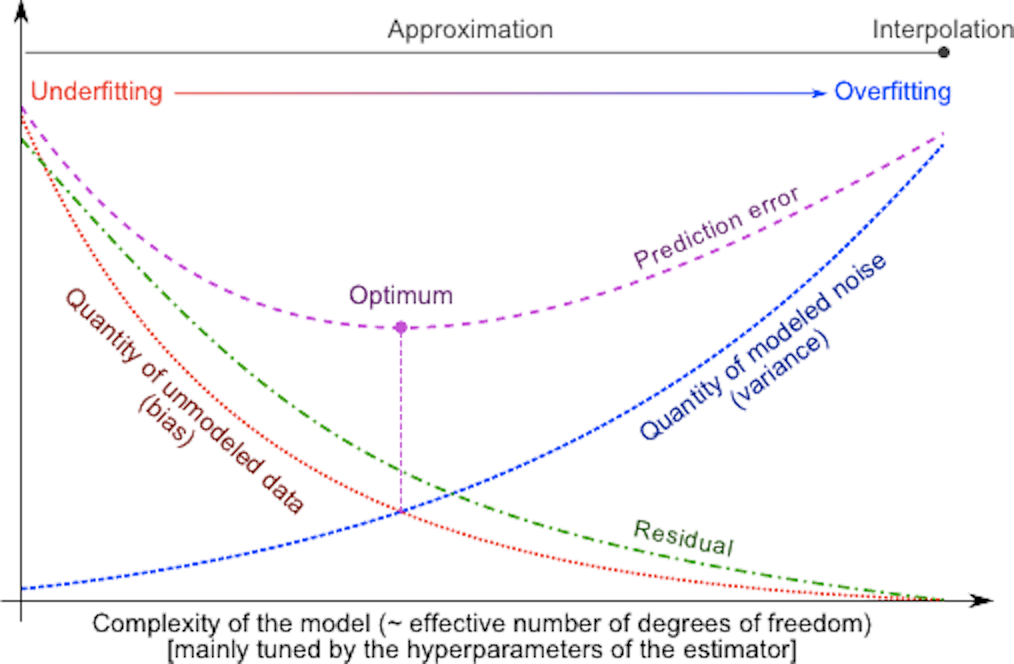
\includegraphics[scale=0.3]{../plots/variance_bias.png}
	\caption{Bias-variance trade-off. Figure showing the bias (red graph). variance (blue graph) and MSE (purple graph) as functions of the complexity of the model. Figure taken from \url{https://www.reddit.com/r/mlclass/comments/mmlfu/a_nice_alternative_explanation_of_bias_and/}}
	\label{fig:variance_bias}
\end{figure}

As we can see from the figure, the bias decreases and the variance increases as the model gets more complex. The MSE is minimized when $\sigma^2=\text{bias}$. 

\subsubsection{R$^2$ score function} \label{sec:R2}
The R$^2$ score function is a measure of how close the data are to the fitted regression line, and is a widely used quantity within statistics. [http://blog.minitab.com/blog/adventures-in-statistics-2/regression-analysis-how-do-i-interpret-r-squared-and-assess-the-goodness-of-fit]

It is defined by how much of the variation that is not explained by the model, i.e, 
\begin{equation*}
\text{R}^2=1-\frac{\text{Explained variation}}{\text{Total variation}}
\end{equation*}
where the explained variation is the MSE and the total variation is given by
\begin{equation*}
\text{Total variation}=\frac{1}{N}\sum_{i=1}^N(y_i-\bar{y})^2.
\end{equation*}

The fraction is always between 0 and 1, it is 0 if the model does not explain any of the variations and 1 if it explains all variations. In that manner, the higher fraction the better score. Since we subtract it from 1 in the total definition, we should fight for a low R$^2$ score. It is in entirety given by
\begin{equation}
R^2(\vec{y},\tilde{\vec{y}})=1-\frac{\sum_{i=1}^N(y_i-\tilde{y})^2}{\sum_{i=1}^N(y_i-\bar{y})^2}.
\end{equation}